\chapter{Общая ценность, аффилированные сигналы}


\section{Напоминалка по теории вероятностей}



\begin{mydef}
Индикатором события $ A $ называется случайная величина, которая равна 1, если $ A $ произошло и 0, если $ A $ не произошло. Обозначают индикатор $ A $ так: $ 1_{A} $.
\end{mydef}

Проверьте, что вы понимаете, что $ \E(1_{A})=\P(A) $.

С помощью индикаторов легко определить условное ожидание:

\begin{mydef}
Если $ \P(A)>0 $, то условным ожидание случайной величины $ X $ при условии события $ A $ называют число:
\[ \E(X|A):=\frac{\E(X\cdot 1_{A})}{\P(A)} \]
\label{posit_condition}
\end{mydef}

Если вам знакомо альтернативное определение условного ожидания, убедитесь, что оно совпадает с этим на паре примеров. Альтернативное определение основано на идее: условное ожидание считается так же, как и безусловное, только вместо безусловной вероятности используется условная.

\begin{myex} Задан закон распределения случайной величины $X$:


\begin{tabular}{c|cccc}
Prob & 0.1 & 0.2 & 0.3 & 0.4 \\ 
\hline 
$X$ & 6 & 2 & 3 & 1 \\ 
\end{tabular} 

Найдите $ \E(X|X>2) $.

Решение:

$\P(X>2)=0.4$

Составляем табличку для $ X\cdot 1_{X>2} $:

\begin{tabular}{c|cccc}
Prob & 0.1 & 0.2 & 0.3 & 0.4 \\ 
\hline 
$1_{X>2}$ & 1 & 0 & 1 & 0 \\ 
$X\cdot 1_{X>2}$ & 6 & 0 & 3 & 0 \\ 
\end{tabular} 

Находим $ \E(X\cdot 1_{X>2})=1.5 $. Значит $ \E(X|X>2)=1.5/0.4=3.75 $

\end{myex}


\begin{myex} Пусть $ X $ распределено экспоненциально с параметром $ \lambda=1 $, т.е. функция плотности $ X $ при $ t\geq 0 $ имеет вид: 
\[ p_{X}(t)=e^{-t} \]
Найдите $ \E(X|X<5) $.

Решение. Находим $ \P(X<5)=\int_{0}^{5}e^{-x}dx=1-e^{-5} $. Затем $ \E(X\cdot 1_{X<5})=\int_{0}^{5} xe^{-x}dx=1-6e^{-5} $. И, следовательно, $ \E(X|X<5)=\frac{e^{5}-6}{e^{5}-1} $

\end{myex}


Часто приходится иметь дело с условным ожиданием виде $ \E(Y|X=x) $. В случае, когда $ X $ дискретна и $ \P(X=x)>0 $ мы без проблем применяем определение \ref{posit_condition}. Однако, если, $ X $ непрерывна и $ \P(X=x)=0 $, у нас возникают проблемы. Впрочем, если $ \P(X\in [x;x+\Delta x])>0$, то наши проблемы легко решаются:
\begin{mydef}
Если $ \P(X\in [x;x+\Delta x])>0 $, то мы определяем условное ожидание $ \E(Y|X=x) $ по формуле:
\begin{equation}
\E(Y|X=x):=\lim_{\Delta x\to 0}\E(Y|X\in [x;x+\Delta x])
\end{equation}
\end{mydef}

Для практических вычислений мы редко (почти никогда в этих лекциях) будем пользоваться определением. Нам будет достаточно четырех свойств:

\begin{itemize}
\item Мат. ожидание суммы равно сумме мат. ожиданий
\begin{equation}
\E(X+Y|A)=\E(X|A)+\E(Y|A)
\end{equation}
\item Константу можно выносить за знак мат. ожидания
\begin{equation}
\E(cX|A)=c\E(X|A)
\end{equation}
\item Значения известной случайной величины можно подставлять:
\begin{equation}
\E(f(X,Y)|X=x)=\E(f(x,Y)|X=x)
\end{equation}
\item Если случайная величина $ X $ и событие $ A $ независимы, то
\begin{equation}
\E(X|A)=\E(X)
\end{equation}

\end{itemize}

Для величин имеющих совместную функцию плотности можно указать способ считать $ \E(Y|X=x) $ без предельного перехода:
\begin{myth} Если пара случайных величин $ X $ и $ Y $ имеет совместную функцию плотности $ f(x,y) $, то 
\begin{equation}
\E(Y|X=x)=\int_{-\infty}^{+\infty}yf(y|x)dy
\end{equation}
\end{myth}

\begin{proof}
\begin{multline}
\E(Y|X\in [x;x+\Delta x])=\frac{\E(Y1_{X\in[x;x+\Delta x]})}{\P(X\in[x;x+\Delta x])}=\frac{\int_{-\infty}^{\infty}\int_{x}^{x+\Delta x} y f(x,y)dx dy }{f_{X}(x)\cdot \Delta x+o(\Delta x)}= \\
=\frac{\int_{-\infty}^{\infty}y\int_{x}^{x+\Delta x}  f(x,y)dx dy }{f_{X}(x)\cdot \Delta x+o(\Delta x)}=\frac{\int_{-\infty}^{\infty}y (f(x,y)\Delta x +o(\Delta x) ) dy }{f_{X}(x)\cdot \Delta x+o(\Delta x)}= \\
=\int_{-\infty}^{\infty}y \frac{f(x,y)\Delta x +o(\Delta x) }{f_{X}(x)\cdot \Delta x+o(\Delta x)} dy 
\end{multline}

При $ \Delta x\to 0 $ указанный интеграл стремится к $ \int_{-\infty}^{+\infty}yf(y|x)dy $.
\end{proof}













\section{Большая сила о-малых!}

В теории вероятностей часто возникает примерно такая задача:

Известна функция плотности случайной величины $ X $, $ p_{X}(t) $. Также известно, как $ Y $ выражается через $ X $, т.е. известно, что $ Y=f(X) $. Причем функция $ f $ --- монотонная и дифференцируемая. Нужно найти функцию плотности $ Y $, $ p_{Y}(t) $.

Есть два способа решения.

Первый --- стандартный, без о-малых и их силы. Нужно знать только, что функция плотности --- это производная от функции распределения:

\[ p_{Y}(y)=\frac{d\P(Y\leq y)}{dy}=\frac{d\P(X\leq f^{-1}(y))}{dy}=p_{X}(f^{-1}(y))\cdot \frac{df^{-1}(y)}{dy} \]

Или, если считать, что $ y=f(x) $:

\begin{equation}
\frac{dy}{dx}p_{Y}(y)=p_{X}(x)
\end{equation}

\begin{myex} Пусть $ X $ имеет функцию плотности $ p_{X}(x)=2x $ на отрезке $ [0;1] $ и $ Y=X^{3} $. Найдите функцию плотности $ Y $.

Решение: Здесь $ y=x^{3} $, значит $ y'=3x^{2} $ и $ x=y^{1/3} $. Значит:
\begin{equation}
3x^{2}p_{Y}(y)=2x
\end{equation}

Подставляем вместо $ x=y^{1/3} $:
\begin{equation}
3y^{2/3}p_{Y}(y)=2y^{1/3}
\end{equation}

Итого:
\begin{equation}
p_{Y}(y)=\frac{2}{3}y^{-1/3}
\end{equation}
\end{myex}

Теперь магия о-малых \index{О-малые}!

Какой смысл в функции плотности? Вероятность того, что $ X $ лежит в отрезке небольшой длины примерно равна произведению длины этого отрезка на значение плотности:

\begin{equation}
\P(X\in [x;x+\Delta x])\approx p(x)\Delta x
\end{equation}

Здесь $ \Delta x $ --- это небольшое число. Если быть точным, то:
\begin{equation}
\P(X\in [x;x+\Delta x])=p_{X}(x)\Delta x+o(\Delta x)
\end{equation}


На всякий случай,
\begin{itemize}
\item $ o(\Delta x) $ --- это такая функция от $ \Delta x $, что:
\begin{equation}
\lim_{\Delta x\to 0} \frac{o(\Delta x)}{\Delta x}=0
\end{equation}
\item $ o(1) $ --- это такая функция от $ \Delta x $, что 
\begin{equation}
\lim_{\Delta x \to 0} o(1)=0
\end{equation}


\end{itemize}
 


Поскольку $ f $ монотонная, то событию $X\in [x;x+\Delta x]  $ соответствует событие $Y\in [y;y+\Delta y]$, где конечно, $ y=f(x) $ и $ \Delta y= f(x+\Delta x)-f(x) $. 

Аналогично:
\begin{equation}
\P(Y\in [y;y+\Delta y])=p_{Y}(y)\Delta y+o(\Delta y)
\end{equation}

Приравниваем две вероятности:
\begin{equation}
p_{X}(x)\Delta x+o(\Delta x)=p_{Y}(y)\Delta y+o(\Delta y)
\end{equation}

Делим на $ \Delta x $:
\begin{equation}
p_{X}(x)+\frac{o(\Delta x)}{\Delta x}=p_{Y}(y)\frac{\Delta y}{\Delta x}+\frac{o(\Delta y)}{\Delta x}
\end{equation}

Устремляем о-малое к нулю и по определению о-малого получаем:
\begin{equation}
p_{X}(x)=p_{Y}(y)\frac{dy}{dx}
\end{equation}

Продолжаем осваивать большую силу о-малых!

Пусть $ X_{1} $, \ldots, $ X_{n} $ --- имеют регулярную функцию распределения $ F() $ на $ [0;1] $ и независимы. Напомним, что мы вводили обозначения $ Y_{1} $, $ Y_{2} $, \ldots, $ Y_{n-1} $ --- это величины $ X_{2} $, $ X_{3} $, \ldots, $ X_{n} $, отсортированные в порядке убывания. В частности, $ Y_{1}=\max\{X_{2},\ldots,X_{n}\} $ --- наибольшая ставка сделанная всеми игроками кроме первого.

\begin{myex} Найдите функцию плотности $ Y_{1} $.

Решение. Прежде чем доставать из ножен о-малые вспомним два простых факта:

\begin{equation}
\P(X_{1}\leq x)=F(x)
\end{equation}

\begin{equation}
\P(X_{1}\in [x_{1};x_{2}])=F(x_{2})-F(x_{1})
\end{equation}


%В аукционе первой цены судьба первого игрока зависит от $ X_{1} $ и $ Y_{1} $\ldots

Вместо плотности $ p_{Y_{1}}(z) $ мы ищем вероятность $ \P(Y_{1}\in [z;z+\Delta z]) $. При маленьких $ \Delta z $ вероятность и плотность связаны:
\begin{equation}
\P(Y_{1}\in [z;z+\Delta z])\approx p_{Y_{1}}(z)\Delta z
\end{equation}


Расчехлим о-малые:

\begin{equation}
\P(X_{2}<X_{1}|X_{1}\in [z;z+\Delta z])=F(z)+o(1)
\end{equation}

Чуть-чуть помедитируйте над этим равенством. При $ \Delta z\to 0 $ правая и левая части становятся похожи на $ F(z) $. Значит верное равенство.

А теперь мы одним махом выпишем ответ!

Что значит $ Y_{1}\in [z;z+\Delta z] $? Это означает, что одна из величин $ X_{i} $ попала в этот интервал. У нас есть $ (n-1) $ возможностей выбрать эту одну. А остальные $ (n-2) $ случайные величины должны быть меньше избранной! Смотрите на ответ:

\begin{equation}
\P(Y_{1}\in [z;z+\Delta z])=(n-1)\cdot (F(z+\Delta z)-F(z)) \cdot (F(z)+o(1))^{n-2}
\end{equation}

По сомножителям:
\begin{itemize}
\item $ (n-1) $ --- это число способов выбрать ту случайную величину, которая будет максимумом. Скажем мы выбрали $ X_{3} $
\item $ F(z+\Delta z)-F(z) $ --- это вероятность того, что $ X_{3} $ попадет в интервал $ [z;z+\Delta z] $.
\item $ F(z)+o(1)=\P(X_{i}<X_{3}|X_{3}\in [z;z+\Delta z]) $
\end{itemize}

Чтобы получить функцию плотности: делим на $ \Delta z $ и устремляем $ \Delta z $ к нулю!

\begin{equation}
p_{Y_{1}}(z)=(n-1)\cdot f(z)\cdot F(z)^{n-2}
\end{equation}


На всякий случай напомню стандартный способ без о-малых:
\begin{multline}
p_{Y_{1}}(z)=\frac{d\P(Y_{1}\leq z)}{dz}=\frac{d \P(X_{2}<z\cap\ldots\cap X_{n}<z)}{dz}=\\
=\frac{dF(z)^{n-1}}{dz}=(n-1)f(z)F(z)^{n-2}
\end{multline}
\end{myex}



Если при поиске отдельной функции плотности можно обойтись без о-малых, то при переходе к совместной функции плотности о-малые впереди на лихом коне!

\begin{myex}
Найдите совместную функцию плотности для пары  $ Y_{1} $ и $ Y_{3} $.

Вместо плотности легче искать вероятность:

\begin{equation}
 \P(Y_{1}\in [w;w+\Delta w] \cap Y_{3} \in [z+\Delta z] )=p(w,z)\Delta w\Delta z+o(dwdz)
\end{equation}


Что значит $ Y_{1} \in [w;w+\Delta w] \cap Y_{3} \in [z+\Delta z]$? Это означает, что одна из величин $ X_{2} $, \ldots, $ X_{n} $ попала в $ [w;w+\Delta w] $. У нас есть $ (n-1) $ возможностей выбрать эту одну. Еще одна попала в $ [z;z+\Delta z] $. Эту одну можно выбрать $ (n-2) $ способом. Еще одна попала между ними, т.е. в интервал $ [w+o(1);z+o(1)] $. Эту одну можно выбрать $ (n-3) $ способами. Оставшиеся $ (n-4) $ случайные величины должны быть меньше $ Y_{3} $, т.к. лежать в интервале $ [0;w+o(1)] $:

\begin{multline}
\P(Y_{1}\in [w;w+\Delta w] \cap Y_{3}\in [z;z+\Delta z] ) =\\
= (n-1)(n-2)(n-3) (F(w+\Delta w)-F(w)) (F(z+\Delta z)-F(z))\cdot \\
\cdot (F(z)-F(w)+o(1)) (F(z)+o(1))^{n-4}
\end{multline}

На всякий случай объясняем по сомножителям:
\begin{itemize}
\item $(n-1)  $ --- это число способов выбрать ту случайную величину, которая будет максимумом. Скажем мы выбрали $ X_{3} $
\item $ (n-2) $ --- это число способов выбрать $ Y_{3} $ среди оставшихся. Скажем мы выбрали $ X_{7} $.
\item $ (n-3) $ --- это число способов выбрать $ Y_{2} $. Ее надо оговаривать особо, т.к. она должна лечь между $ Y_{1} $ и $ Y_{3} $. Пусть это оказалась $ X_{9} $.
\item $(F(w+\Delta w)-F(w))$ --- это $ \P(X_{3}\in [w;w+\Delta w]) $
\item $(F(z+\Delta z)-F(z))$ --- это $ \P(X_{7}\in [z;z+\Delta z] ) $
\item $(F(w)-F(z)+o(1))$ --- это $ \P(X_{9}\in [w+o(1);z+o(1)] ) $
\item $ (F(z)+o(1))^{n-4} $ --- это вероятность того, что оставшиеся $ X_{i} $ меньше $ X_{7} $
\end{itemize}

Делим на $ \Delta w $, $ \Delta z $ и устремляем их к нулю.

\begin{equation}
p_{Y_{1},Y_{3}}(w,z)=(n-1)(n-2)(n-3)f(z)f(w)(F(w)-F(z))F(z)^{n-4}
\end{equation}

\end{myex}








 

\section{Старые формулы на вероятностном языке}


\begin{quotation}
Сова стала объяснять, что такое Необходимая или Соответствующая Спинная Мускулатура. Она уже объясняла это когда-то Пуху и Кристоферу Робину и с тех пор ожидала удобного случая, чтобы повторить объяснения, потому что это такая штука, которую вы спокойно можете объяснять два раза, не опасаясь, что кто-нибудь поймёт, о чём вы говорите.

Алан Милн в переводе Бориса Заходера.
\end{quotation}

Мы быстро повторим то, что сделали на первой лекции:
\begin{myth}
Если сигналы совпадают с ценностями, т.е. $ X_{i}=V_{i} $, то ожидаемая прибыль первого игрока может быть записана как:
\begin{enumerate}
\item $\pi_{1}(x,b(a))=(x-b(a))\cdot (F(a))^{n-1}$, если $ X_{i} $ независимы
\item $\pi_{1}(x,b(a))=(x-b(a))\cdot \P(Y_{1}<a|X_{1}=x)$, если $ X_{i} $ зависимы
\end{enumerate}
\end{myth}

\begin{proof}
Для аукциона первой цены:
\begin{equation}
Pay_{1}=Bid_{1}\cdot 1_{W_{1}}
\end{equation}

Значит:
\begin{equation}
Profit_{1}=X_{1}\cdot 1_{W_{1}}-Pay_{1}=(X_{1}-Bid_{1})\cdot 1_{W_{1}}
\end{equation}



\begin{multline}
\E(Profit_{1}|X_{1}=x ; Bid_{1}=b_{1})=\\
=\E((X_{1}-Bid_{1})\cdot 1_{W_{1}}|X_{1}= x ; Bid_{1}=b_{1})=\\
= (x-b_{1})\E(1_{W_{1}}|X_{1}=x ; Bid_{1}=b_{1})=\\
=(x-b_{1})\P(W_{1}|X_{1}=x ; Bid_{1}=b_{1})
\end{multline}

Озаботимся величиной $ \P(W_{1}|X_{1}=x ; Bid_{1}=b_{1}) $. Если ценности независимы, то:
\begin{multline}
\P(W_{1}|X_{1}=x ; Bid_{1}=b_{1})=\P(W_{1}|Bid_{1}=b_{1})= \\
=\P(Bid_{2}<Bid_{1}\cap \ldots ; Bid_{n}<Bid_{1}|Bid_{1}=b_{1})=\\
=\P(Bid_{2}<b_{1}\cap \ldots ; Bid_{n}<b_{1})=\\
=\P(Bid_{2}<b_{1})^{n-1}=\P(b(X_{2})<b_{1})^{n-1}
\end{multline}

Дальше чудо-замена $ b_{1}=b(a) $. Уточняем: $ b_{1} $ --- константа, $ a $ --- константа, $ b() $ --- неизвестная, но детерминистическая функция.

\begin{equation}
\P(b(X_{2})<b_{1})^{n-1}=\P(b(X_{2})<b(a))^{n-1}=\P(X_{2}<a)^{n-1}=(F(a))^{n-1}
\end{equation}

Итого, для аукциона первой цены с независимыми ценностями:
\begin{equation}
\pi_{1}(x,b(a))=(x-b(a))\cdot (F(a))^{n-1}
\end{equation}

Что меняется, если ценности зависимы?

Единственное отличие состоит в том, что:
\begin{equation}
\P(W_{1}|X_{1}=x ; Bid_{1}=b_{1}) \neq \P(W_{1}|Bid_{1}=b_{1})
\end{equation}

На этот раз вероятность упрощается не так сильно:
\begin{multline}
\P(W_{1}|X_{1}=x ; Bid_{1}=b_{1})=\\
=\P(Bid_{2}<Bid_{1}\cap \ldots \cap Bid_{n}<Bid_{1}|X_{1}=x ; Bid_{1}=b_{1})=\\
=\P(Bid_{2}<b_{1}\cap \ldots \cap Bid_{n}<b_{1}|X_{1}=x)=\\
=\P(b(X_{2})<b_{1}\cap \ldots \cap b(X_{n})<b_{1}|X_{1}=x)
\end{multline}

И еще чуть-чуть после чудо-замены:
\begin{multline}
\P(b(X_{2})<b_{1}\cap \ldots \cap b(X_{n})<b_{1}|X_{1}=x)=\\
\P(b(X_{2})<b(a)\cap \ldots \cap b(X_{n})<b(a)|X_{1}=x)=\\
\P(X_{2}<a\cap \ldots \cap X_{n}<a|X_{1}=x)
\end{multline}

А эту вероятность можно посчитать, если известна совместная функция плотности ценностей. С использованием обозначения $ Y_{1}=\max\{X_{2},\ldots, X_{n}\} $ можно записать ее короче:
\begin{equation}
\P(X_{2}<a\cap \ldots \cap X_{n}<a|X_{1}=x)=\P(Y_{1}<a|X_{1}=x)
\end{equation}

Итого, для аукциона первой цены с зависимыми ценностями:
\begin{equation}
\pi_{1}(x,b(a))=(x-b(a))\cdot \P(Y_{1}<a|X_{1}=x)
\end{equation}
\end{proof}

А сейчас мы увидим, как с помощью мат. ожидания записать уже знакомые нам вещи. А именно:

\begin{myth} Если предпосылки теоремы об одинаковой доходности выполнены, то:
\label{probabilistic_interpretation}
\begin{itemize}
\item Для произвольного аукциона $ q(x)=\P(Y_{1}<x) $
\item Для произвольного аукциона $ pay(x)=\E(Y_{1}\cdot 1_{Y_{1}<x}) $
\item Для аукциона первой цены $ b(x)=\E(Y_{1}|Y_{1}<x) $ 
\end{itemize}
\end{myth}

\begin{proof}

Первое. Из предпосылки о том, что товар достается тому покупателю, у которого выше ценность немедленно следует, что $ q(x)=\P(Y_{1}<x) $.

Второе. В одном из упражнений первой лекции мы установили:
\begin{equation}
pay(x)=pay(0)+\int_{0}^{x}t \cdot \frac{dq(t)}{dt}\cdot dt
\end{equation}

Если предпосылки теоремы об одинаковой доходности выполнены, то:
\begin{equation}
pay(x)=\int_{0}^{x}t \cdot \frac{dq(t)}{dt}\cdot dt
\end{equation}


Вспоминаем, что:
\begin{equation}
q(x)=F(x)^{n-1}
\end{equation}

Стало быть
\begin{equation}
\frac{dq(x)}{dx}=(n-1)f(x)F(x)^{n-2}
\end{equation}

И!!! Мы видим, что это есть функция плотности $ Y_{1} $!!!:
\begin{equation}
\frac{dq(x)}{dx}=p_{Y_{1}}(x)
\end{equation}

Т.е. для любого аукциона подходящего в теорему об одинаковой доходности:
\begin{equation}
pay(x)=\int_{0}^{x}t \cdot p_{Y_{1}}(t)\cdot dt=\E(Y_{1}\cdot 1_{Y_{1}<x})
\end{equation}



Третье. На аукционе первой цены:
\begin{equation}
pay(x)=b(x)\cdot q(x)
\end{equation}

Пользуемся первыми двумя результатами и получаем:
\begin{equation}
\E(Y_{1}1_{Y_{1}<x})=b(x)\cdot \P(Y_{1}<x)
\end{equation}

Отсюда немедленно следует, что:
\begin{equation}
b(x)=\frac{\E(Y_{1}1_{Y_{1}<x})}{\P(Y_{1}<x)}=\E(Y_{1}|Y_{1}<x)
\end{equation}



\end{proof}





 

\section{Просто разные примеры}


\begin{myex} Потренируем о-малую мускулу. Найдем равновесие Нэша в аукционе третьей цены\index{Аукцион третьей цены}. Его правила таковы. Есть $ n $ игроков, они одновременно делают ставки. Товар получает тот, кто назвал самую высокую ставку, но платит от не свою ставку, а третью по величине ставку. Предполагаем, что ценность и сигнал --- это одно и то же, т.е. $ V_{i}=X_{i} $, а сами сигналы $ X_{i} $ независимы и имеют регулярное распределение на $ [0;1] $.


Мы только что доказали, что при выполнении теоремы об одинаковой доходности:
\begin{equation}
pay_{1}(x)=\E(Y_{1}\cdot 1_{Y_{1}<x})=\int_{0}^{x}tp_{Y_{1}}(t)dt
\end{equation}

Из этого следует, что:
\begin{equation}
\frac{dpay_{1}(x)}{dx}=xp_{Y_{1}}(x)
\end{equation}


С другой стороны на аукционе третьей цены первый игрок платит третью по величине ставку, значит вторую по величине ставку игроков не считая себя.

\begin{equation}
pay_{1}(x)=\E(Pay_{1}|X_{1}=x)=\E(b(Y_{2})\cdot 1_{W_{1}}|X_{1}=x)
\end{equation}

Если мы предположим, что в равновесии функция $ b() $ строго возрастает, то 
\begin{equation}
W_{1}=\{b(X_{1})>b(X_{2})\cap \ldots\cap  b(X_{1})>b(X_{n})\}=\{X_{1}>Y_{1}\}
\end{equation} 

Т.к. $ X_{i} $ независимы, нашу функцию выплат можно записать с помощью безусловного мат. ожидания:
\begin{equation}
pay_{1}(x)=\E(b(Y_{2})\cdot 1_{Y_{1}<X_{1}}|X_{1}=x)=\E(b(Y_{2})\cdot 1_{Y_{1}<x})
\end{equation}

Судя по формуле нам нужна совместная функция плотности $ Y_{1} $ и $ Y_{2} $. О-малые приходят на помощь:

\begin{equation}
p(y_{1},y_{2})=(n-1)(n-2)f(y_{1})f(y_{2})F(y_{2})^{n-3}
\end{equation}

Следует уточнить, что эта формула верна при $0<y_{2}<y_{1}<1$. При остальных $ y_{1} $ и $ y_{2} $ плотность равна нулю.

Для нахождения математического ожидания выписываем страшный двойной интеграл:
\begin{multline}
pay_{1}(x)=\E(b(Y_{2})\cdot 1_{Y_{1}<x})=\int_{0}^{1}\int_{0}^{y_{1}} b(y_{2})1_{y_{1}<x} p(y_{1},y_{2})dy_{2}dy_{1}=\\
=\int_{0}^{x}\int_{0}^{y_{1}} b(y_{2})p(y_{1},y_{2})dy_{2}dy_{1}=\\
=\int_{0}^{x}\int_{0}^{y_{1}} b(y_{2}) (n-1)(n-2)f(y_{1})f(y_{2})F(y_{2})^{n-3} dy_{2}dy_{1}=\\
(n-1)(n-2)\int_{0}^{x}f(y_{1})\int_{0}^{y_{1}} b(y_{2}) f(y_{2})F(y_{2})^{n-3} dy_{2}dy_{1}
\end{multline}

Конечно, интегрировать это мы не будем. Мы наоборот, возьмем производную по $ x $ два раза. Берем производную первый раз:
\begin{equation}
\frac{dpay_{1}(x)}{dx}=(n-1)(n-2)f(x)\int_{0}^{x} b(y_{2}) f(y_{2})F(y_{2})^{n-3} dy_{2}
\end{equation}

С другой стороны, 
\begin{equation}
\frac{dpay_{1}(x)}{dx}=xp_{Y_{1}}(x)=x(n-1)f(x)(F(x))^{n-2}
\end{equation}

После сокращения $ (n-1) $ и $ f(x) $ мы получили уравнение:
\begin{equation}
(n-2)\int_{0}^{x} b(y_{2}) f(y_{2})F(y_{2})^{n-3} dy_{2}=x(F(x))^{n-2}
\end{equation}

Чтобы избавиться от интеграла берем еще раз производную по $ x $ от обеих частей.
\begin{equation}
(n-2) b(x) f(x)F(x)^{n-3}=F(x)^{n-2}+(n-2)xf(x)F(x)^{n-3}
\end{equation}

Выражаем $ b(x) $:
\begin{equation}
b(x)=\frac{F(x)}{(n-2)f(x)}+x
\end{equation}

При равномерном распределении наша формула превращается в:
\begin{equation}
b(x)=\frac{n-1}{n-2}x
\end{equation}

Она возрастает по $ x $, значит теорему об одинаковой доходности действительно можно было применять.
\end{myex}


\begin{myex} Общая ценность. 

Предположим, что на аукционе первой цены продается участок с домом. Торгуются два игрока. Ценность участка с домом одинакова для обоих игроков. Только они ее не совсем полностью знают. Один игрок хорошо разбирается в домах, а второй --- в земельных участках. Т.е. Природа сообщает первому игроку ценность дома, а второму --- ценность участка. 

Введем обозначения:

\begin{itemize}
\item $ V_{i} $ --- случайная величина, ценность товара для игрока $ i $
\item $ X_{i} $ --- случайная величина, сигнал от Природы, который получает игрок $ i $
\end{itemize}

В нашем случае: $ V_{1}=V_{2}=X_{1}+X_{2} $ --- это ценности товара, а $ X_{1} $ --- сигнал, часть ценности, известная первому игроку и $ X_{2} $ --- сигнал, часть ценности, известная второму игроку.

Предположим, что $ X_{i} $ независимы и равномерны на $ [0;1] $. Найдите равновесие Нэша.

Решение:

В этом случае прибыль равна:

\begin{equation}
Profit_{1}=(V_{1}-Bid_{1})\cdot 1_{W_{1}}
\end{equation}

Находим нашу детерминистическую функцию:

\begin{multline}
\E(Profit_{1}|X_{1}=x; Bid_{1}=b_{1})=\\
=\E((x+X_{2})-b_{1})\cdot 1_{W_{1}}|X_{1}=x; Bid_{1}=b_{1})=\\
=(x-b_{1})\P(W_{1}|X_{1}=x; Bid_{1}=b_{1})+\E(X_{2}\cdot 1_{W_{1}}|X_{1}=x; Bid_{1}=b_{1})
\end{multline}


Здесь нужно быть очень аккуратным т.к. $ \E(X\cdot Y) $ в общем случае не совпадает с $ \E(X)\cdot \E(Y) $!

В силу независимости $ X_{i} $ и того, что $ Bid_{2}=b(X_{2}) $ упрощаем $\P(W_{1}|X_{1}=x ; Bid_{1}=b_{1})$:
\begin{multline}
\P(W_{1}|X_{1}=x; Bid_{1}=b_{1})=\\
=\P(Bid_{2}<Bid_{1}|X_{1}=x; Bid_{1}=b_{1})=\P(Bid_{2}<b_{1})
\end{multline}

Вспомнив чудо-замену $ b_{1}=b(a) $ получаем:
\begin{equation}
\P(Bid_{2}<b_{1})=\P(b(X_{2})<b(a))=\P(X_{2}<a)=F(a)
\end{equation}

Упрощаем: $ \E(X_{2}\cdot 1_{W_{1}}|X_{1}=x; Bid_{1}=b_{1}) $:
\begin{multline}
\E(X_{2}\cdot 1_{W_{1}}|X_{1}=x; Bid_{1}=b_{1})=\E(X_{2}\cdot 1_{Bid_{2}<Bid_{1}}|X_{1}=x; Bid_{1}=b_{1})=\\
=\E(X_{2}\cdot 1_{b(X_{2})<b_{1}}|X_{1}=x)=\E(X_{2}\cdot 1_{b(X_{2})<b_{1}})
\end{multline}

В последнем переходе мы использовали то, что $ X_{1} $ и $ X_{2} $ независимы.

И, чудо-замена,

\begin{equation}
\E(X_{2}\cdot 1_{b(X_{2})<b_{1}})=\E(X_{2}\cdot 1_{b(X_{2})<b(a)})=\E(X_{2}\cdot 1_{X_{2}<a})=\int_{0}^{a}tf(t)dt
\end{equation}

Собираем все вместе:

\begin{equation}
\pi_{1}(x,b(a))=(x-b(a))F(a)+\int_{0}^{a}tf(t)dt
\end{equation}

Берем производную по $ a $: 
\begin{equation}
-b'(a)F(a)+(x-b(a))f(a)+af(a)=0
\end{equation}

Т.к. мы ищем равновесие Нэша, оптимальное $b_{1}=b(x)  $, и значит, оптимальное $ a=x $:

\begin{equation}
-b'(x)F(x)+(x-b(x))f(x)+xf(x)=0
\end{equation}

В случае равномерных ценностей:
\begin{equation}
-b'(x)x+(x-b(x))+x=0
\end{equation}

Это линейное дифференциальное уравнение, общее решение имеет вид $ b(x)=x+\frac{c}{x} $. Единственное ограниченное на $ [0;1] $ решение --- это $ b(x)=x $. Почему нас не интересуют неограниченные решения? Потому, что оно заведомо не оптимально. Если стратегия $ b(x) $ принимает значения больше единицы, то стратегия $ \min\{b(x),1\} $ окажется лучше. Стратегия $ b(x) $ с положительной вероятностью приводит к ситуации, когда мы выигрываем товар, но обязаны заплатить за него сумму выше 1, т.е. мы получаем отрицательный выигрыш. Стратегия $ \min\{b(x),1\} $ этого недостатка лишена, а во всем прочем точно копирует стратегию $ b(x) $.

\end{myex}


\begin{myex} Кнопочный аукцион с зависимыми ценностями.
У нас имеется три игрока, $ V_{1}=V_{2}=V_{3}=X_{1}+X_{2}+X_{3} $, ценности независимы и равномерны на $ [0;1] $. Найдите равновесные Нэша и средний доход продавца.

Самое сложное --- это понять, что является здесь стратегией игрока. Напомню правила. Текущая цена равна времени прошедшему с момента начала аукциона. В начале все игроки жмут свои кнопки. Каждый сам решает, когда ему отпустить кнопку. Как только кнопку отпускает предпоследний игрок, аукцион оканчивается. Победителем считается тот, кто продолжает давить. Он получает товар, по текущей цене на конец аукциона. Во время аукциона игроки знают кто и когда его покидает. Стратегия игрока может учитывать эту информацию. Если ценности зависимы, так оно и окажется.

Рассмотрим первого игрока. Стратегия должна говорить игроку: до которого времени давить кнопку, если никто другой не вышел, и до которого времени давить кнопку, если один другой игрок вышел на цене $ p $. При всем при этом стратегия может учитывать известное игроку значение $ X_{1} $. В результате стратегия игрока в симметричном случае описывается двумя (!) функциями $ (b^{3}(x), b^{2}(x,p)) $:
\begin{itemize}
\item $ b^{3}(x) $ --- до которого времени давить кнопку, если в игре 3 игрока
\item $ b^{2}(x,p) $ --- до которого времени давить кнопку, если в игре 2 игрока, и один ушел на цене $ p $
\end{itemize}


Сейчас мы предъявим равновесные стратегии, а затем докажем, что они действительно равновесные.

Пусть:
\begin{itemize}
\item $ b^{3}(x)=x+x+x=3x$
\item $ b^{2}(x,p)=x+x+\frac{p}{3}=2x+\frac{p}{3}$
\end{itemize}

Откуда взялись эти стратегии? 


Первая, $ b^{3}() $, получилась подстановкой $ x $ в платежную функцию вместо каждого $ X_{i} $. 

Чтобы понять вторую, $ b^{2}(x,p) $, давайте еще раз вспомним, что такое равновесие Нэша.  Равновесие Нэша --- это набор стратегий, такой что игрокам не выгодно в одиночку их менять, даже если они расскажут друг другу о своих стратегиях. Т.е. при поиске равновесия Нэша можно считать стратегии общеизвестными! 

Теперь допустим, что текущая цена равна $ p $, и остальные два игрока используют функцию $ b^{3}() $. И вдруг кто-то из них выходит. Это означает, что для него $ b^{3}(x)=p $. Значит для уходящего игрока $ x=\frac{p}{3} $. В равновесии Нэша этот вывод могут сделать все игроки! Т.е. можно восстановить сигнал $ x $ уходящего игрока, зная цену на которой он вышел. И мы вводим новую функцию $ b^{2}(x,p) $, в которой сигнал ушедшего игрока выражен через $ p $, а сигналы остающихся игроков по-прежнему заменены на одно и то же $ x $.

Чем они хороши?

Сначала определим, в каком порядке будут выходить игроки, если все используют указанную стратегию. Сначала выйдет тот игрок, у кого минимальное значение $ b^{3}(X_{i}) $. Поскольку $ b^{3}() $ строго возрастающая функция первым выйдет игрок с минимальным $ X_{i} $. Допустим это произошло на цене $ p $. Следующим игроком из двух оставшихся выйдет тот, у кого $ b^{2}(X_{i},p) $ меньше. Но $ b_{2}(x,p) $ строго возрастает по $ x $, а значение $ p $ одинаковое, значит вторым выйдет тот из оставшихся игроков, у кого $ X_{i} $ меньше. Мораль. Если игроки используют эти стратегии, то они выходят в порядке возрастания ценностей и товар получает тот, у кого $ X_{i} $ наибольшее. Это хорошее свойство указанной стратегии, но еще не доказательство оптимальности.

Почему же они все-таки равновесны?

Рассматриваем ситуацию, когда все игроки кроме первого используют указанную стратегию. Мы сейчас посчитаем какой выигрыш получает первый игрок, если тоже использует указанную стратегию и сколько он получит, если отклонится.

Пусть первый игрок также использует стратегию $ (b^{3}(x), b^{2}(x,p)) $. Возможно две ситуации: 
\begin{itemize}
\item Первый игрок выигрывает аукцион. 

Это происходит, если его ценность выше других, т.е. $ X_{1}>Y_{1} $. В этом случае первый выход из игры происходит при цене $ b^{3}(Y_{2}) $, а второй --- при цене $ b^{2}(Y_{1},b^{3}(Y_{2})) $. Значит первый игрок заплатит $ b^{2}(Y_{1},b^{3}(Y_{2})) $. И выигрыш первого игрока равен:
\begin{multline}
V_{1}-b^{2}(Y_{1},b^{3}(Y_{2}))=X_{1}+X_{2}+X_{3}-b^{2}(Y_{1},b^{3}(Y_{2}))=\\
=X_{1}+Y_{1}+Y_{2}-Y_{1}-Y_{1}-Y_{2}=X_{1}-Y_{1}>0 
\end{multline}
Если игрок захочет отклонится, т.е. не выиграть аукцион, то он получит 0. Значит отклоняться не выгодно.

\item Первый игрок проигрывает аукцион. 

Это происходит, если его ценность не максимальная, т.е. $ X_{1}<Y_{1} $. В этом случае его доход равен 0. Сколько игрок получит, если захочет отклонится, т.е. выиграть?
\begin{multline}
 V_{1}-b^{2}(Y_{1},b^{3}(Y_{2}))=X_{1}+X_{2}+X_{3}-b^{2}(Y_{1},b^{3}(Y_{2}))=\\
 =X_{1}+Y_{1}+Y_{2}-Y_{1}-Y_{1}-Y_{2}=X_{1}-Y_{1}<0 
\end{multline}
Отклоняться не выгодно.
\end{itemize}


Считаем среднюю выручку продавца:
\begin{equation}
\E(R)=\E(b^{2}(Y_{1},b^{3}(Y_{2}))|X_{1}>Y_{1})=\E((2Y_{1}+Y_{2})|X_{1}>Y_{1})=\ldots=1.25
\end{equation}

Замечания:
\begin{itemize}
\item При определении стратегий была важна связь между $ X_{i} $ и $ V_{i} $, но не совместная функция плотности $ X_{i} $. В решении равномерность распределения не использовалась!
\item Если после окончания игры игроки раскроют значения своих $ X_{i} $ друг другу, то никто не пожалеет о выбранной стратегии. Проигравшие не жалеют, т.к. при известных $ X_{i} $ им ничего не светит. Выигравший не жалеет, т.к. при фиксированных стратегиях других игроков выиграть за меньшую сумму он не мог.
\item Аукцион как и раньше очень сильно похож на аукцион второй цены
\end{itemize}




\end{myex}



\section{Супермодулярные функции}

Введем более короткие обозначения для максимума и минимума:

\begin{equation}
x\wedge y\wedge z =\min\{x,y,z\}
\end{equation}

\begin{equation}
x\vee y\vee z =\max\{x,y,z\}
\end{equation}

Запомнить эти обозначения легко поняв их происхождение. Кто-то когда-то давно заметил, что минимум и максимум нескольких чисел ведут себя точно так же, как пересечение и объединение множеств:

Убедитесь, что для множеств верно:

\begin{equation}
(A \cap B)\cup C=(A\cup C)\cap (B\cup C)
\end{equation}

А для чисел верно:
\begin{equation}
(a \wedge b)\vee c=(a\vee c)\wedge (b\vee c)
\end{equation}

Совпадение это не случайно. Если какая-то формула для множеств верна, то она верна и для подмножеств числовой прямой вида $ (-\infty;t] $. А на таких подмножествах аналогия совершенно прямая: если $ A=(-\infty;a] $ и $ B=(-\infty;b] $, то $ A\cup B= (-\infty;a\vee b] $ и $ A\cap B=(-\infty;a\wedge b] $.

Докажите, что, например, верны формулы:

\begin{equation}
1_{A}\wedge 1_{B}=1_{A\cap B}
\end{equation}

\begin{equation}
1_{A}\vee 1_{B}=1_{A\cup B}
\end{equation}


%Эти значки называются мит и джойн (?)\ldots

Аналогичные операции применяются и к векторам:

\begin{mydef} Если $ \vec{x}=(x_{1},\ldots, x_{n}) $ и $ \vec{y}=(y_{1},\ldots, y_{n}) $, то:
\begin{equation}
\vec{x}\wedge\vec{y}=(x_{1}\wedge y_{1}, \ldots, x_{n}\wedge y_{n}) 
\end{equation}

\begin{equation}
\vec{x}\vee\vec{y}=(x_{1}\vee y_{1}, \ldots, x_{n}\vee y_{n}) 
\end{equation}

\end{mydef}


В экономическом моделировании то там, то сям возникают супермодулярные функции:

\begin{mydef} Функция $ f() $ называется \indef{супермодулярной}\index{Супермодулярная функция}, если для любых $ \vec{x} $ и $ \vec{y} $
\begin{equation}
f(\vec{x}\wedge\vec{y})+f(\vec{x}\vee\vec{y})\geq f(\vec{x})+f(\vec{y})
\end{equation}

\end{mydef}

\begin{myex} Функция $ f(x_{1},x_{2})=x_{1} $ является супермодулярной. Действительно, левая часть равна:
\begin{equation}
f(\vec{x}\wedge\vec{y})+f(\vec{x}\vee\vec{y})=x_{1}\wedge y_{1}+x_{1}\vee y_{1}=x_{1}+y_{1}
\end{equation}
Правая часть равна:
\begin{equation}
f(\vec{x})+f(\vec{y})=x_{1}+y_{1}
\end{equation}
\end{myex}

\begin{myex} Функция $ f(x)=x^{3} $ является супермодулярной:
\begin{multline}
f(x\wedge y)+f(x \vee y)=(x\wedge y)^{3}+(x\vee y)^{3}=x^{3}\wedge y^{3} + x^{3}\vee y^{3}=\\
=x^{3}+y^{3}=f(x)+f(y)
\end{multline}
\end{myex}

\begin{myex} Функция $ f(x_{1},x_{2})=-x_{1}x_{2} $ не является супермодулярной:
\begin{equation}
f((1,2)\wedge (2,1))+f((1,2)\vee (2,1))=f(2,2)+f(1,1)=-4-1=-5
\end{equation}
\begin{equation}
f(1,2)+f(2,1)=-2-2=-4
\end{equation}


\end{myex}




\begin{myth} Если у функции $ f $ существуют вторые производные, то она является супермодулярной если и только если для $ i\neq j $:
\label{supermod_crit}
\begin{equation}
\frac{\partial^{2}f}{\partial x_{i}\partial x_{j}}\geq 0
\end{equation}
\end{myth}

Сначала мы докажем, что эта теорема верна для функции двух переменных.
\begin{proof} Случай двух переменных.

Рассмотрим функцию $ f(x,y) $ и четыре точки на плоскости, $ a'>a $ и $ b'>b $:


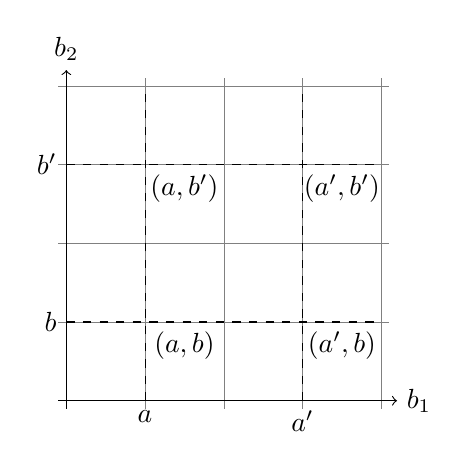
\begin{tikzpicture}
    \draw[style=help lines,color=gray] (-0.1,-0.1) grid (4.1,4.1);
    \draw[->] (-0.1,0) -- (4.2,0) node[right] {$b_1$};
    \draw[->] (0,-0.1) -- (0,4.2) node[above] {$b_2$};
    \draw[color=black,dashed] (1,0)--(1,4) ;
    \draw[color=black,dashed] (3,0)--(3,4) ;
    \draw[color=black,dashed] (0,1)--(4,1) ;
    \draw[color=black,dashed] (0,3)--(4,3) ;
	\node[below] at (1,0) {$a$};
	\node[below] at (3,0) {$a'$};
	\node[left] at (0,1) {$b$};
	\node[left] at (0,3) {$b'$};
	\node at (1.5,0.7) {$(a,b)$};
	\node at (3.5,0.7) {$(a',b)$};
	\node at (1.5,2.7) {$(a,b')$};
	\node at (3.5,2.7) {$(a',b')$};
\end{tikzpicture}

Применяя определение супермодулярности к паре $ (a,b') $ и $ (a',b) $ мы получаем:
\begin{equation}
f((a',b)\wedge(a,b')) + f((a',b)\vee(a,b'))\geq f(a',b) + f(a,b')
\end{equation}

Применительно к нашим точкам:
\begin{equation}
f(a,b)+f(a',b')\geq f(a',b)+f(a,b')
\end{equation}

Или:
\begin{equation}
f(a',b')-f(a',b)\geq f(a,b')-f(a,b)
\end{equation}

Что можно озвучить словами так: разность $ f(x,b')-f(x,b) $ растет по $ x $ при $ b'>b $.

%Следовательно, $ \ln (f(x,b')/f(x,b)) $ растет по $ x $ при $ b'>b $.

Значит при $ b'>b $:
\begin{equation}\label{first_deriv}
\frac{\partial }{\partial x}(f(x,b')-f(x,b))=\frac{\partial }{\partial x}f(x,b')-\frac{\partial }{\partial x} f(x,b) \geq 0
\end{equation}

По определению, вторая производная, это:
\begin{equation}
\frac{\partial^{2}}{\partial x \partial y}f(x,b)=\lim_{\Delta b\to 0}\frac{\frac{\partial }{\partial x}f(x,b+\Delta b)-\frac{\partial }{\partial x} f(x,b)}{\Delta b}
\end{equation}
Если взять $ b'=b+\Delta b $ и $ \Delta b>0 $ мы получаем положительные числитель и знаменатель. Значит и сама вторая производная будет положительной.

В обратную сторону. Если вторая производная всюду неотрицательна, то первая производная разности растет по $ b $, т.е. мы получаем формулу \ref{first_deriv}. Остальные переходы равносильны.

\end{proof}


Чтобы получить доказательство для произвольного случая нам понадобится такая теорема полезная и сама по себе:
\begin{myth}
Функция $ f(x_{1},\ldots,x_{n}) $ является супермодулярной если и только если она является супермодулярной функцией от любых двух своих переменных при фиксированных значениях остальных переменных. 
\end{myth}

\begin{proof}

Мы докажем теорему для функции трех переменных. В общем случае доказательство ничем не сложнее, просто навешивается куча индексов.

Итак, пусть у нас есть супермодулярная функция трех аргументов, $ f(a,b,c) $. 

Заметим, что рассмотрев ее как функцию двух аргументов, зафиксировав любой третий мы получим снова супермодулярную функцию. Например, если $ g(a,b):=f(a,b,c) $, то $ g $ --- супермодулярна:

\begin{multline}
g((x_{1},x_{2})\vee (y_{1},y_{2}))+g((x_{1},x_{2})\wedge (y_{1},y_{2}))=\\
f((x_{1},x_{2},c)\vee (y_{1},y_{2},c))+f((x_{1},x_{2},c)\wedge (y_{1},y_{2},c))\geq \\
f((x_{1},x_{2},c))+f((y_{1},y_{2},c))=g(x_{1},x_{2})+g(y_{1},y_{2})
\end{multline}

В обратную сторону чуть посложнее\ldots Пусть при рассмотрении любых двух переменных мы получаем супермодулярную функцию.

Рассмотрим две точки, $(a',b',c) $ и $ (a,b,c') $. Штрихованная переменная больше, $ a'>a $, $ b'>b $, $ c'>c $. 

Получаем:
\begin{multline}
f((a',b',c)\vee (a,b,c'))+f((a',b',c)\wedge (a,b,c'))-f(a',b',c)-f(a,b,c')=\\
f(a',b',c')+f(a,b,c)-f(a',b',c)-f(a,b,c')=\\
f(a',b',c')+f(a,b,c)-f(a',b,c)-f(a,b',c')+\\
+[f(a',b,c)-f(a',b,c)]+[f(a',b,c')-f(a',b,c')]=\\
[f(a',b',c')+f(a',b,c)-f(a',b,c')-f(a',b',c)]+\\
+[f(a,b,c)+f(a',b,c')-f(a',b,c)-f(a,b,c')]\geq 0
\end{multline}

При доказательстве для $ n>3 $ можно пользоваться предположением индукции, т.е. тем, что для $ n-1 $ теорема уже доказана.
\end{proof}

Нам супермодулярные функции понадобятся для описания зависимости между сигналами  $X_{i}$. Мы хотим, чтобы сигналы были связаны положительно между собой. Например, если выставлен на торги хороший лот, то все участники считают его хорошим. А выставлен плохой --- все более или менее видят, что он плох. Более формально:

%Мы предположим, что игрок не полностью знает ценность товара для себя. Т.е. каждый игрок получает от Природы сигнал $ X_{i} $. Отныне $ X_{i} $ --- это не ценность товара для игрока $ i $!

\begin{mydef}
Случайные величины $ X_{1} $, \ldots, $ X_{n} $ с совместной функцией плотности $ f(x_{1},\ldots,x_{n}) $ называются \indef{аффилированными}\index{Аффилированные случайные величины}, если $ \ln(f(\vec{x})) $ --- супермодулярная функция.
\end{mydef}

Чуть позже (теорема \ref{prop_affiliated}) мы докажем, что из аффилированности случайных величин $ X $ и $ Y $ следует например, что:
\begin{enumerate}
\item $ Cov(X,Y)\geq 0 $
\item Функция $g(x)= \E(Y|X=x) $ неотрицательно зависит от $ x $
\end{enumerate}

В силу того, что логарифм произведения равен сумме логарифмов, это определение эквивалентно следующему:
\begin{mydef}
Случайные величины $ X_{1} $, \ldots, $ X_{n} $ с совместной функцией плотности $ f(x_{1},\ldots,x_{n}) $ называются \indef{аффилированными}\index{Аффилированные случайные величины}, если

\begin{equation}
f(\vec{x}\wedge\vec{y})\cdot f(\vec{x}\vee\vec{y})\geq f(\vec{x})\cdot f(\vec{y})
\end{equation} 
\end{mydef}




%Упражнение:




% Известно, что аффилированы случайные величины $ X_{1} $, \ldots, $ X_{n} $. Верно ли, что аффилированы случайные величины $ X_{1} $, \ldots, $ X_{n-1} $?


%\begin{myth}
%Если аффилированы $ X_{1} $, \ldots, $ X_{n} $, то аффилированы $ X_{1} $, $ Y_{1} $, $ Y_{2} $, \ldots, $ Y_{n-1} $
%\end{myth}

%\begin{proof}
%\ldots
%\end{proof}

\section{Задачи}
\begin{enumerate}

\item Пусть $ A $ и $ B $ --- это события. Верно ли, что $ \E(1_{A}|B)=\P(A|B) $?

\item Пусть $ A $ и $ B $ --- это независимые события. Верно ли, что $ \E(1_{A}|B)=\E(1_{A})  $?

\item С помощью о-малых найдите:

\begin{enumerate}
\item функцию плотности минимума остальных ставок, $ p_{Y_{n-1}}(t) $
\item функцию плотности $ p_{Y_{6}}(t) $
\item совместную функцию плотности $ p_{Y_{1},Y_{n-1}}(a,b) $
\item совместную функцию плотности $ p_{Y_{3},Y_{6}}(a,b) $
\item совместную функцию плотности $ p_{Y_{n-2},Y_{n-1}}(a,b) $
\item совместную функцию плотности $ p_{X_{1},Y_{1}}(a,b) $
\end{enumerate} 

\item Рассмотрим аукцион первой цены двух игроков. Ценности независимы и имеют функцию плотности $f(t)=2t  $ на $ [0;1] $. 

Найдите:
\begin{enumerate}
\item Равновесие Нэша, т.е. детерминистические стратегии $ b(x) $
\item Детерминистическую функцию $ pay_{1}(x) $
\item Детерминистическую функцию $ \widehat{pay_{1}}(b) $
\item Детерминистическую функцию $ q_{1}(x) $
\item Детерминистическую функцию $ \widehat{q_{1}}(b) $
\item Функцию распределения случайной величины $ Pay_{1} $
\item $ \E(Pay_{1}) $, $ Cov(Pay_{1},Pay_{2}) $, $ Var(Pay_{1}) $
\item Функцию распределения случайной величины $ R $
\item $ \E(R) $, $ Var(R) $, $ Cov(R,Pay_{1}) $
\item Тонкая разница! Если применить детерминистическую функцию $ pay_{1}(x) $ к случайной величине $ X_{1} $, то мы получим случайную величину $ pay_{1}(X_{1}) $. Временно обозначим ее $ L_{1} $ (и забудем это обозначение после этого упражнения). Найдите функцию распределения $ L_{1} $, $ \E(L_{1}) $, $ Var(L_{1}) $, $ Cov(L_{1},L_{2}) $

\end{enumerate}

\item Предположим, что на аукционе первой цены продается участок с домом. Торгуются два игрока. Природа сообщает первому игроку ценность дома, $ X_{1} $, а второму --- ценность участка, $ X_{2} $. При этом ценности игроков определяются по формулам: $ V_{1}=X_{1}+0.5X_{2} $ --- первому важнее дом, $ V_{2}=0.5X_{1}+X_{2} $ --- второму важнее участок. Ценности независимы и равномерны на $ [0;1] $. Найдите равновесие Нэша.

\item Сколько функций потребуется (и от каких переменных каждая из них зависит) чтобы описать стратегию в симметричном равновесии Нэша в кнопочном аукционе с 4-мя игроками? С 5-ю? С $ n $ игроками?

\item Сколько функций потребуется (и от каких переменных каждая из них зависит) чтобы описать стратегию в несимметричном равновесии Нэша в кнопочном аукционе с 4-мя игроками? С 5-ю? С $ n $ игроками?

\item Рассмотрим кнопочный аукцион с тремя игроками. Каждый игрок знает своё $ X_{i} $, а ценности определяются по правилу:
\begin{equation}
V_{1}=X_{1}+X_{2}\cdot X_{3} \\
V_{2}=X_{2}+X_{1}\cdot X_{3} \\
V_{3}=X_{3}+X_{1}\cdot X_{2} \\
\end{equation}
Сигналы $ X_{i} $ независимы и имеют равномерное распределение на $ [0;1] $. Найдите равновесие Нэша и средний доход продавца.

\item Найдите $ (1,2,3)\wedge (5,0,2) $ и $ (1,2,3)\vee (5,0,2) $

\item Являеются ли супермодулярными функции:
\begin{enumerate}
\item $ f(x_{1},\ldots,x_{n})=x_{1}+\ldots+x_{n} $
\item $ f(x_{1},\ldots,x_{n})=x_{1}\cdot \ldots \cdot x_{n} $ при положительных $ x_{i} $
\item $ f(a,b,c)=a\wedge b\wedge c $
\item $ f(a,b,c)=a\vee b\vee c $
\end{enumerate}

\item Существует ли функция одной переменной не являющаяся супермодулярной?

\item Верно ли, что $ X_{i} $ аффилированы если:

\begin{enumerate}
\item $ X_{1} $, \ldots, $ X_{n} $ --- независимы
\item $ f(x,y)=x+y $ при $ x,y\in [0;1] $
\item $ f(x,y)=\frac{1+4xy}{2} $ при $ x,y\in [0;1] $
\end{enumerate}

\item Пара случайных величин $ X $ и $ Y $ имеет совместное нормальное распределение с корреляцией $ \rho $. При каких $ \rho $ они будут аффилированы?

\end{enumerate}


\section{Решения задач}
\begin{enumerate}

\item Да. $ \E(1_{A}|B)=\E(1_{A}1_{B})/\P(B)=\P(A\cap B)/\P(B)=\P(A|B) $

\item Да. $ \E(1_{A}|B)=\P(A|B)=\P(A)=\E(1_{A})$ 

\item 
\begin{enumerate}
\item $ p_{Y_{n-1}}(t)=(n-1)f(t)(1-F(t))^{n-2} $
\item $ p_{Y_{6}}(t)=(n-1)f(t)C^{5}_{n-1}(1-F(t))^{5}(F(t))^{n-7} $
\item $ p_{Y_{1},Y_{n-1}}(a,b)=(n-1)(n-2)f(a)f(b)(F(a)-F(b))^{n-3} $
\item $ p_{Y_{3},Y_{6}}(a,b)=(n-1)(n-2)C_{n-3}^{2}C_{n-5}^{2}f(a)f(b) (F(b))^{n-7}(1-F(a))^{2}(F(a)-F(b))^{2} $
\item $ p_{Y_{n-2},Y_{n-1}}(a,b)=(n-1)(n-2)f(a)f(b)(1-F(a))^{n-3} $
\item $ p_{X_{1},Y_{1}}(a,b)=f(a)(n-1)f(b)(F(b))^{n-2} $
\end{enumerate} 


\item 

\begin{enumerate}
\item Стратегии $ b(x) $ мы уже искали в предыдущей домашней работе, $ b(x)=\frac{2}{3}x $
\item Функцию $ pay_{1}(x) $ проще всего найти через теорему \ref{probabilistic_interpretation}:
\begin{equation}
pay_{1}(x)=\int_{0}^{x}t(n-1)f(t)(F(t))^{n-2}dt=\frac{2}{3}x^{3}
\end{equation}
\item Функция $ \widehat{q_{1}}(b) $ --- это вероятность того, что первый выиграет, если поставит $ b $. Значит:
\begin{multline}
\widehat{q_{1}}(b)=\P(Bid_{2}<b)=\P\left(\frac{2}{3}X_{2}<b\right)=\\
=\P\left( X_{2}<\frac{3}{2}b\right)=F\left(\frac{3}{2}b\right)=\left(\frac{3}{2}b\right)^{2}
\end{multline}
\item Ищем $ \widehat{pay_{1}}(b) $:
\begin{equation}
\widehat{pay_{1}}(b)=\E(b\cdot 1_{Bid_{2}<b})=b\cdot \P(Bid_{2}<b)=b\left(\frac{3}{2}b\right)^{2}
\end{equation}
\item Функция $ q_{1}(x) $ --- это вероятность того, что первый выиграет при ценности $ x $, значит $ q_{1}(x)=x^{2} $
\item Cлучайная величина $ Pay_{1} $ --- интересный зверь. Она не является ни дискретной, ни непрерывной. Заметим, что в равновесии с вероятностью $ 0.5 $ первый проигрывает аукцион и не платит ничего. Значит у функции распределения скачок высотой 0.5 в точке $ t=0 $! А в остальных точках --- она непрерывна. Замечаем, что область значений $ Pay_{1} $ --- отрезок $ [0;2/3] $\ldots

Более детально рассматриваем точки $ t\in (0;2/3) $
\begin{multline}
\P(Pay_{1}\leq t)=\P(Pay_{1}\leq t \cap X_{1}>X_{2})+\P(Pay_{1}\leq t \cap X_{1}<X_{2})=\\
=\P(Pay_{1}\leq t \cap X_{1}>X_{2})+\P(X_{1}<X_{2})=\\
=\P(Pay_{1}\leq t \cap X_{1}>X_{2})+0.5
\end{multline}

Считаем первую вероятность отдельно:
\begin{multline}
\P(Pay_{1}\leq t \cap X_{1}>X_{2})=\P(\frac{2}{3}X_{1}\leq t \cap X_{1}>X_{2})=\\
\P(X_{1}\leq 1.5t \cap X_{1}>X_{2})=\int_{0}^{1.5t}\int_{0}^{x_{1}} 2x_{1}2x_{2}dx_{2}dx_{1}=\frac{81}{32}t^{4} 
\end{multline}

Итого, получаем функцию распределения:
\begin{equation}
F_{Pay_{1}}(t)=
\begin{cases} 
0, t<0 \\
0.5+\frac{81}{32}t^{4}, t\in [0;2/3] \\
1, t>2/3 \\
\end{cases}
\end{equation}

Функции плотности у $ Pay_{1} $ нет! Функция распределения разрывна. Тем не менее выпишем производную:
\begin{equation}
f_{Pay_{1}}(t)=0.5d(0)+\frac{81}{8}t^{3}
\end{equation}
В начале формулы идет некое мифическое $ 0.5d(0) $ --- это просто условная запись. Она нужна чтобы помнить, что у  $ F(t) $ в точке $ t=0 $ был скачок высотой $ 0.5 $.


\item $ \E(Pay_{1}) $, , $ Var(Pay_{1}) $

Считаем мат. ожидание. Это легко. От дискретной части появляется $ 0\cdot 0.5 $. От непрерывной --- интеграл.
\begin{equation}
\E(Pay_{1})=0\cdot 0.5+\int_{0}^{2/3}t\cdot \frac{81}{8}t^{3} dt=\ldots=4/15
\end{equation}

Для дисперсии нам нужно:
\begin{equation}
\E(Pay_{1}^{2})=0^{2}\cdot 0.5+\int_{0}^{2/3}t^{2}\cdot \frac{81}{8}t^{3} dt=\ldots=4/27
\end{equation}

Дисперсия равна:
\begin{equation}
Var(Pay_{1})=\E(Pay_{1}^{2})-\E(Pay_{1})^{2}=4/27-(4/15)^{2}=52/675
\end{equation}


Два игрока никогда не платят одновременно, поэтому $ Pay_{1}\cdot Pay_{2} $ тождественно равно нулю. Отсюда:
\begin{multline}
Cov(Pay_{1},Pay_{2})=\E(Pay_{1}Pay_{2})-\E(Pay_{1})\E(Pay_{2})=\\
=0-(4/15)^{2}
\end{multline}
\item Cлучайная величина $ R$ --- это не что иное, как максимум из ставок:
\begin{equation}
R=\max\left\{ \frac{2}{3}X_{1},\frac{2}{3}X_{2} \right\}=\frac{2}{3}\max\{X_{1},X_{2}\}
\end{equation}
Функция распределения:
\begin{multline}
F_{R}(t)=\P(R\leq t)=\P\left(\frac{2}{3}\max\{X_{1},X_{2}\}\leq t\right)=\\
=\P\left(X_{1}<\frac{3}{2}t \cap X_{2}<\frac{3}{2}t\right)=F\left(\frac{3}{2}t\right)^{2}=\left(\frac{3}{2}t\right)^{4}
\end{multline}
Это непрерывная случайная величина, и у нее есть функция плотности:
\begin{equation}
f_{R}(t)=4\left(\frac{3}{2}t\right)^{3}\frac{3}{2}
\end{equation}

\item Для нахождения $ \E(R) $, $ Var(R) $, $ Cov(R,Pay_{1}) $ вспоминаем, что $ R=Pay_{1}+Pay_{2} $.
\begin{equation}
\E(R)=\E(Pay_{1}+Pay_{2})=2\E(Pay_{1})
\end{equation}
\begin{equation}
Var(R)=Var(Pay_{1})+Var(Pay_{2})+2Cov(Pay_{1},Pay_{2})
\end{equation}

\begin{multline}
Cov(R,Pay_{1})=Cov(Pay_{1}+Pay_{2},Pay_{1})=\\
=Var(Pay_{1})+Cov(Pay_{2},Pay_{1})
\end{multline}
\item В нашем случае $ L_{1}=\frac{2}{3}X_{1}^{3} $.

Функция распределения:
\begin{multline}
F_{L_{1}}(t)=\P(L_{1}<t)=\P\left(\frac{2}{3}X_{1}^{3}<t\right)=\\
=\P(X_{1}<(1.5t)^{1/3})=F((1.5t)^{1/3})=(1.5t)^{2/3}
\end{multline}

В данном случае речь идет о непрерывной случайной величине, у нее есть функция плотности:
\begin{equation}
f_{L_{1}}(t)=1.5\frac{2}{3}(1.5t)^{-1/3}
\end{equation}

Мат. ожидание:
\begin{equation}
\E(L_{1})=\int_{0}^{1}\frac{2}{3}t^{3}2tdt=\frac{4}{15} 
\end{equation}

Дисперсия:
\begin{equation}
Var(L_{1})=\E(L_{1}^{2})-\E(L_{1})^{2}=\frac{1}{9}-\left(\frac{4}{15}\right)^{2}=\frac{1}{25}
\end{equation}

Поскольку $ X_{1} $ и $ X_{2} $ независимы, $ pay(X_{1}) $ и $ pay(X_{2}) $ тоже независимы, и $ Cov(L_{1},L_{2})=0 $
\end{enumerate}

Заметим, что $ \E(Pay_{1})=\E(pay_{1}(X_{1})) $, но $Var(Pay_{1})\neq Var(pay(X_{1}))$! Ковариации также различаются\ldots Т.е. $ Pay_{1} $ и $ pay_{1}(X_{1}) $ --- это разные случайные величины!


\item От рассмотренного примера отличается только коэффициентом $ 0.5 $ перед $ \E(X_{2}1_{W_{1}}|\ldots) $. Значит финальное дифф. уравнение имеет вид:
\begin{equation}
-b'(x)F(x)+(x-b(x))f(x)+0.5\cdot xf(x)=0
\end{equation}
При равномерном распределении:
\begin{equation}
-b'(x)x+(x-b(x))+0.5\cdot x=0
\end{equation}

Подбираем сразу линейное решение, получаем $ b(x)=0.75x $

\item Для четырех. $ b^{4}(x) $, $ b^{3}(x,p_{4}) $, $ b^{2}(x,p_{3},p_{4}) $ (названия переменных объясняются соглашением, что $ p_{i} $ --- это моменты выхода игроков в порядке убывания)

Для пяти. $ b^{5}(x) $, $ b^{4}(x,p_{5}) $, $ b^{3}(x,p_{4},p_{5}) $, $ b^{2}(x,p_{3},p_{4},p_{5}) $

Для $ n $ игроков. Нужна $ (n-1) $ функция, $ b^{n}(x) $, $ b^{n-1}(x,p_{n}) $, \ldots, $ b^{2}(x,p_{3},\ldots,p_{n}) $

\item Начнем все-таки с трех. Заметим, что у каждого игрока свои стратегии! Например, рассмотрим первого:
\begin{enumerate}
\item $b_{1}^{3}(x)$ --- до какого момента давить на кнопку, если в игре 3 игрока.
\item $b_{1}^{2:-2}(x,p) $ --- до какого момента давить на кнопку, если в игре 2 игрока и первым вышел второй.
\item $b_{1}^{2:-3}(x,p) $ --- до какого момента давить на кнопку, если в игре 2 игрока и первым вышел третий.
\end{enumerate}

Для четырех (функции описывают, до какого момента давить на кнопку)
\begin{enumerate}
\item $b_{1}^{4}(x)$ --- если все четверо в игре
\item $b_{1}^{3:2}(x,p) $ --- если вышел только второй на цене $ p $
\item $b_{1}^{3:3}(x,p) $ --- если вышел только третий на цене $ p $
\item $b_{1}^{3:4}(x,p) $ --- если вышел только четвертый на цене $ p $

\item $b_{1}^{2:2,3}(x,p_{3},p_{4}) $ --- если сначала вышел второй, на цене $ p_{4} $, а затем --- третий, на цене $ p_{3} $
\item $b_{1}^{2:2,4}(x,p_{3},p_{4}) $
\item $b_{1}^{2:3,4}(x,p_{3},p_{4}) $
\item $b_{1}^{2:3,2}(x,p_{3},p_{4}) $
\item $b_{1}^{2:4,2}(x,p_{3},p_{4}) $
\item $b_{1}^{2:4,3}(x,p_{3},p_{4}) $
\end{enumerate}
Итого: $1+3+6=10$ функций.

Для пяти: $1+4+12+24=41$ функция.

Для произвольного $ n $: $ C_{n-1}^{1}1!+C_{n-1}^{2}2!+C_{n-1}^{3}3!+C_{n-1}^{4}4!+\ldots C_{n-1}^{n-2}(n-2)! $


\item Сначала равновесие. Первая функция --- $ b^{3}(x)=x+x^{2} $. Со второй чуть посложнее\ldots 
Если игрок вышел на цене $ p $, то $ x+x^{2}=p $. Решаем квадратное уравнение, берем корень из $ [0;1] $:
\begin{equation}
x=\frac{\sqrt{1+4p}-1}{2}
\end{equation}
И получаем:
\begin{equation}
b^{2}(x,p)=x+x\frac{\sqrt{1+4p}-1}{2}=x\frac{\sqrt{1+4p}+1}{2}
\end{equation}

Пусть $ Z_{1} $ --- наибольшая из всех $ X_{i} $, $ Z_{2} $ --- вторая по величине, а $ Z_{3} $ --- самая маленькая. Тогда побеждает игрок с сигналом $ Z_{1} $. При этом он платит $ b^{2}(Z_{2},b(Z_{3}))=Z_{2}+Z_{2}Z_{3} $.

Значит:
\begin{equation}
\E(R)=\E(Z_{2}+Z_{2}Z_{3})=\E(Z_{2})+\E(Z_{2}Z_{3})
\end{equation}

Для их расчета привлекаем банду о-малых. 


Ищем функцию плотности $ Z_{2} $. Три способа выбрать $ Z_{2} $, одна из двух $ X_{i} $ должна быть больше избранной (сомножитель $ (1-t) $), другая --- меньше (сомножитель $ t $):
\begin{equation}
p_{Z_{2}}(t)=3\cdot 2\cdot t(1-t)
\end{equation}

Совместная функция плотности положительна только при $ a>b $ и равна:
\begin{equation}
p_{Z_{2},Z_{3}}(a,b)=6(1-a)
\end{equation}

После интегрирования первой получаем очевидный результат, что мат. ожидание медианы трех равномерных случайных величин равно половине:
\begin{equation}
\E(Z_{2})=\ldots=1/2
\end{equation}

И после интегрирования второй:
\begin{equation}
\E(Z_{2}Z_{3})=\ldots=\frac{3}{20}
\end{equation}

Итого: $ \E(R)=\frac{13}{20} $

\item Ответ: $ (1,2,3)\wedge (5,0,2)=(1,0,2) $ и $ (1,2,3)\vee (5,0,2)=(5,2,3) $

\item К первым двум можно применять теорему \ref{supermod_crit}.
\begin{enumerate}
\item $ \frac{\partial^{2} f}{\partial x_{i}\partial x_{j}}=0 $, супермодулярна
\item $ \frac{\partial^{2} f}{\partial x_{i}\partial x_{j}}>0 $, супермодулярна
\item да, супермодулярна. Достаточно, например, рассмотреть два случая:
\begin{enumerate}
\item $ x_{1}>y_{1} $, $ x_{2}>y_{2} $, $x_{3}>y_{3}$. Здесь $ f(\vec{x}\wedge \vec{y})=f(\vec{y}) $ и $ f(\vec{x}\vee \vec{y})=f(\vec{x}) $ и неравенство выполнено.
\item $ x_{1}>y_{1} $, $ x_{2}>y_{2} $, $x_{3}<y_{3}$ Здесь нужно немного помучиться с рассмотрением разных порядков\ldots
\end{enumerate}
\item нет, не супермодулярна. Например: $ \vec{x}=(3,3,1) $ и $ \vec{y}=(2,2,4) $. Тогда: $ \vec{x}\wedge \vec{y}=(2,2,1) $ и $ \vec{x}\vee\vec{y}=(3,3,4) $. Находим, что: $ f(\vec{x}\wedge \vec{y})=2 $, $ f(\vec{x}\vee \vec{y})=4 $, $ f(\vec{x})=3 $, $ f(\vec{y})=4 $

\end{enumerate}

\item Нет. Если $ x=y $, то $ x\wedge y=x\vee y=x=y $  и $ f(x\wedge y)+f(x\vee y)= f(x)+f(y) $. Если $ x\neq y $, то одно из этих чисел больше, а другое --- меньше. А это значит, что $ x=x\wedge y $ и $ y=x \vee y $. Или наоборот, $ x=x\vee y $ и $ y=x\wedge y $.

\item 
\begin{enumerate}
\item Независимые случайные величины аффилированы: $ \ln(f(x,y,z)=\ln(f(x))+\ln(f(y))+\ln(f(z)) $
\item Если $ f(x,y)=x+y $, то 
\begin{equation}
\frac{\partial^{2} \ln(f)}{\partial x \partial y}=-\frac{1}{(x+y)^{2}}<0
\end{equation}
Значит, величины не аффилированны. Кстати, в этом примере ради интереса можно посчитать ковариацию: $ \E(X)=\E(Y)=7/12 $, $ \E(XY)=1/3 $, $ Cov(X,Y)=-1/144 $.
\item Если  $ f(x,y)=\frac{1+4xy}{2} $, то:
\begin{equation}
\frac{\partial^{2} \ln(f)}{\partial x \partial y}=\ldots=\frac{4}{(1+4xy)^{2}}\geq 0
\end{equation}
Случайные величины аффилированны

\end{enumerate}

\item Для начала заметим, что ответ на вопрос не зависит от мат. ожидания и дисперсии. Это связано с тем, что в силу теоремы \ref{supermod_crit} нужна только неотрицательность смешанной второй производной логарифма плотности при любых $ x $ и $ y $. Выбор мат. ожидания --- это перенос графика плотности вдоль осей, выбор дисперсии --- это растяжение графика плотности вдоль осей. Если была где-то точка с отрицательной второй смешанной производной, то она просто поменяет свои координаты.

Рассматриваем случай с нулевым мат. ожиданием и единичной дисперсией. Ковариационная матрица имеет вид: 
\begin{equation}
S=\left(\begin{array}{cc}
1 & \rho \\
\rho & 1 \\
\end{array} 
\right)
\end{equation}

Функция плотности равна:

\begin{equation}
p(x,y)=\frac{1}{2\pi \det(S)} \exp\left(-\frac{1}{2}(x\; y)S^{-1}(x\; y)^{t}\right)
\end{equation}
После логарифмирования получаем (нам интересна только смешанная вторая производная, поэтому следим только за коэффициентом при $ xy $):

\begin{equation}
\ln (p(x,y))=\ldots+\frac{\rho}{1-\rho^{2}}xy
\end{equation}
Значит двумерное совместное нормальное распределение аффилированно если корреляция неотрицательная.


\end{enumerate}
